% !TEX root = ../main.tex

\section{Project Status}

The status of the project is that we have completed the setup of a VM with
BBR available. This involved configuring a Linux (Ubuntu) VM with an updated
kernel that included the BBR congestion control algorithm. In addition, we
have access to the \texttt{tcp\_bbr.c}\footnote{
\url{http://elixir.free-electrons.com/linux/latest/source/net/ipv4/tcp_bbr.c}}
source, which allows us to modify and recompile the kernel module, if needed.

In addition, we have been able to write an experiment script in Python that
collects data on BBR and CUBIC throughput performance at varying loss rates.
We use MahiMahi\footnote{\url{http://mahimahi.mit.edu/}} as our network
emulator. To setup the experiment, we use a delay shell to simulate a 100ms
delay, a loss shell to control the amount of packet loss, and a link
shell to approximate a 100Mbps link and mimic the conditions of the original
BBR results.

Once the data collection is complete, the script generates a plot of the
performance between BBR and CUBIC.

A preliminary run produced the graph results in Figure~\ref{fig:rebbr8}. We
can see that CUBIC only performs acceptably when the loss rate is extremely
small. At loss rates of 0.01\% and above, CUBIC performance deteriorates.
BBR, on the other hand, is able to deliver a larger percentage of the available
throughput when compared to CUBIC on loss rates as high as 50\%.


\begin{figure}[h]
  \centering
  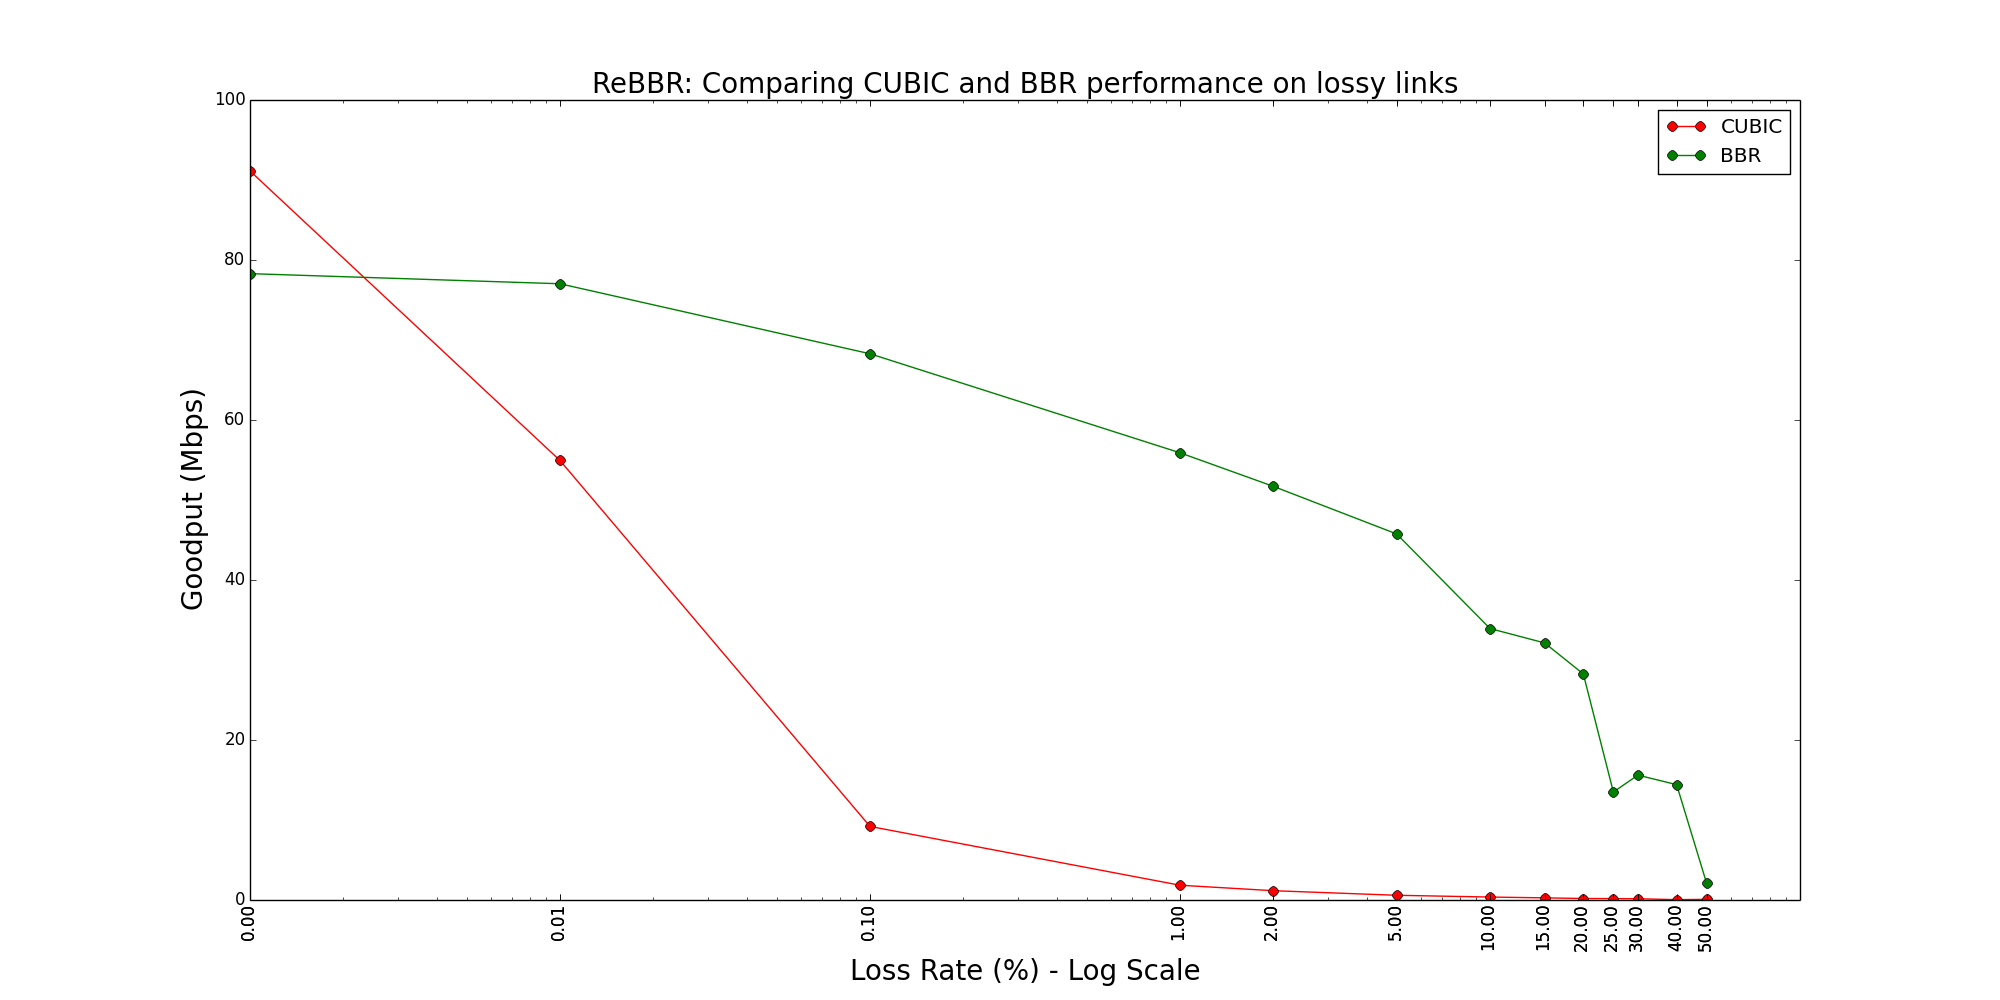
\includegraphics[height=5cm]{./img/rebbr_fig8.png}
  \caption{ReBBR: Throughput vs loss rate comparing CUBIC vs BBR.}
  \label{fig:rebbr8}
\end{figure}


\para{Plan}
Currently, we still have some potential bugs to work out in our experimental
script, and will need to perform a more rigorous experiment of reproducing
the results if Figure~\ref{fig:bbr8} (e.g. more runs on longer traces).
We would then hope to analyze and comment on the results and discrepancies.

Once the primary result has been reproduced, we would like to explore the
different parameters of this experiment, such as which congestion control
algorithms are compared against, the characteristics of the network, and
perhaps the internal parameters of CUBIC if time permits. For example,
we would like to see how BBR compares to other TCP congestion control
algorithms such as TCP VEGAS or TCP NewReno, how BBR behaves on a lossy
cellular link trace compared to CUBIC, or how the total bottleneck bandwidth
available affects the comparison (e.g. running on 1Mbps rather than 100Mbps).

Currently, our experimental scripts are hard-coded for a particular case, and
we will need to make some significant modifications to support exploring more
of these parameters. We likely will not be able to explore all of these
parameters, but hope to evaluate a few in the remainder of the quarter.

% For the remainder of the quarter, we need to make the experiment setup run on
% Google Cloud. Running a machine on Google Cloud costs a few dollars, so for
% convenience and for faster iterating, we have been doing our work in a local
% Linux Ubuntu VM. The next step is to replicate that setup to run successfully
% in the Google Cloud.
%
% We would also like to explore how BBR compares to other modern TCP congestion
% control algorithms such as VEGAS and NEW RENO.
%
% We are also interested on evaluating how does the performance between CUBIC and BBR vary, if at all, when the network
% link is running an order of magnitude slower. For example at 10Mbps, 1Mbps, 0.1Mbps (100kbps) and 0.01Mbps (10kbps).
% Similarly, it would also be interesting to see the variation when the RTT changes by an order of magnitude. For example
% at 0.01s, 0.1s, 1.0s, 10, 60s. Performance on the low bandwidth, high latency links should give insights into
% potential benefits of BBR when deployed over slow 2G cellular links.
%
% Finally, we need to write up our final report discussing the results we found.
%
% Admittedly, this is  quite a bit of material and we'll try to get through as much of it as possible, time permitting.
